\section{Evaluation Design}\label{sec:design}

\subsection{Research Questions}
\begin{itemize}
\item[RQ1)] \emph{Evidence integrity and reproducibility.} Can \sbg{} produce integrity-checked evidence whose analysis is reproducible, and which attacks within the threat model are blocked, detected only, without effect, or successful?
\item[RQ2)] \emph{\ers{} conformance.} Do the \sbg{} estimators and decision procedures satisfy the eight \ers{} properties on real evidence records, and does the property matrix detect defects?
\item[RQ3)] \emph{Observed false-assurance risk.} How often do no-divergence verdicts of plain differential testing and of rule-based gates conceal a labelled behavioural change, and how does this trade off against coverage?
\item[RQ4)] \emph{Incremental value of \cec{} and \ers{}.} At matched coverage, does \cec{}, with or without \ers{} features, lower false-assurance risk or improve probabilistic accuracy relative to coverage-only calibration, the predecessor's gate and random abstention?
\item[RQ5)] \emph{Scope of the evaluation evidence.} Which evaluation settings were actually executed, what does each establish, and what do the five-dataset artifact and the cross-platform runs not establish?
\end{itemize}
RQ1, RQ2 and RQ5 use no labels. RQ3 and RQ4 use construction labels. Table~\ref{tab:design} gives the design of each question.

\begin{table*}[!t]
\caption{Experimental design by research question. All label-dependent analyses use construction labels on development data.}
\label{tab:design}
\centering
\scriptsize
\setlength{\tabcolsep}{2.8pt}
\begin{tabular}{|c|L{2.3cm}|L{2.5cm}|L{1.5cm}|L{2.4cm}|L{2.2cm}|L{2.6cm}|L{1.9cm}|}
\hline
RQ & Objective & Data & Unit & Metrics & Comparators & Analysis & Main limitation \\
\hline
1 & Integrity and reproducible analysis & Attack and probe suites (macOS, Linux); Linux and macOS analysis outputs on the same records & Attack; analysis run & Outcome category; numerical agreement & Pre-hardening suite; other platform & Classification of recorded outcomes; diff of saved outputs & Author-written attacks; Linux run lacks host metadata \\
2 & \ers{} conformance & 312 records $\times$ 6 predictors $\times$ 10 perturbations; 30-pair real-execution analogue & Trial & Pass / fail / N/A; responses beyond tolerance & Fitted model, probe, stub, V7-B recorded and recomputed & Counts from the property matrix; pre/post profile fix & Post-hoc edits; constant gate features \\
3 & Observed risk of rules & 258 labelled pairs & Pair & $\hat\cov$, $\hat\R$, worst case & B1--B6 & Cluster bootstrap (10,000) & Construction labels; one dominant cluster \\
4 & Incremental value & 258 labelled pairs; 85 soft / 61 strict eligible & Pair (out-of-fold) & $\hat\R(c^\ast)$; Brier; log loss; calibration slope & B3, B6, B7, B9; ablations & Grouped 5-fold CV; paired cluster bootstrap; Holm; MDE & Underpowered (MDE $\approx$16\,pp) \\
5 & Scope of evaluation evidence & All settings A--G (Table~\ref{tab:benchmarks}); five-dataset generator code; cross-platform outputs & Setting; record; activity & Executed vs.\ asserted; agreement & Repository reports & Static audit of code, manifests and outputs & No held-out benchmark evaluation exists \\
\hline
\end{tabular}
\end{table*}

\subsection{Evaluation Settings and Evidence Categories}
Breadth is easy to overstate, so we separate seven categories of evaluation evidence and state the status of each (Table~\ref{tab:benchmarks}, Fig.~\ref{fig:landscape}(b)).
\begin{enumerate}
\item[A)] \emph{Real program-pair evaluation.} 312 version pairs executed by the collector: 150 synthetic pairs from 101 programs, 116 pairs derived from 31 QuixBugs programs, and 46 function-level units from 43 BugsInPy bugs in 12 real Python projects. All are development data. Only the synthetic and QuixBugs pairs carry (construction) labels.
\item[B)] \emph{Real-execution perturbation evaluation.} Execution-level analogues of P2, P5 and P6 on 30 pairs drawn from three arms (20 synthetic, 5 QuixBugs negatives, 5 BugsInPy units); 720 trial rows; exploratory.
\item[C)] \emph{Cross-platform systems validation.} The same analysis and post-hoc \ers{} matrix run on macOS and Linux over identical records.
\item[D)] \emph{Security and integrity evaluation.} 25 attacks and probes re-run on macOS at the final commit; 125 Linux probes before the last fix.
\item[E)] \emph{Unit and regression testing.} The implementation's test suite (247 passed, 8 skipped, 2 expected failures, macOS).
\item[F)] \emph{Template-derived artifacts, excluded.} A ``five-dataset'' artifact named after Defects4J, BugsInPy, Bears, BugSwarm and Bugs.jar. A static audit (RQ5) found that its 250 records come from 12 hand-written templates with outcomes assigned from labels and that no benchmark code was executed. Its outcomes were set from labels, its predictor was the activation stub, and it has zero completed human verdicts. It is invalid as external-validation evidence and is a pipeline smoke test that supports no claim.
\item[G)] \emph{Independent outcome adjudication.} Designed and implemented, not executed. Every label in this paper is a construction label.
\end{enumerate}
The study therefore has several distinct evaluation settings, A--E. Apart from the held-out test split described in the results, all of them are single-language (Python), development-exposed and unadjudicated. One evaluation used a held-out test split: a single frozen run on the v8 test split (22 programs, 956 valid pairs). Its pre-declared criterion was not met, and it is not a confirmatory external validation.

\begin{table*}[!t]
\caption{Evaluation landscape. Every row except F and G is an executed setting with machine-readable output. ``Dev.''\ = development data, examined during design. GT = ground truth.}
\label{tab:benchmarks}
\centering
\scriptsize
\setlength{\tabcolsep}{2.4pt}
\renewcommand{\arraystretch}{1.08}
\begin{tabular}{|c|L{2.6cm}|L{2.1cm}|L{0.9cm}|L{1.25cm}|L{1.9cm}|L{2.3cm}|L{1.3cm}|L{3.2cm}|}
\hline
Cat. & Source & Subjects (projects) & Lang. & Executed; OS & Objective & GT provenance & Independent & Main limitation \\
\hline
A & Synthetic pairs & 150 (101 programs) & Python & Yes; one env.\ id & RQ2--RQ4 & Generator labels & No (dev.) & Generated changes; small programs \\
A & QuixBugs~\cite{lin2017quixbugs} buggy/fixed & 31 (1 benchmark, 31 programs) & Python & Yes; one env.\ id & RQ2--RQ4 & Benchmark tests & No (dev.) & Label and evidence share inputs \\
A & QuixBugs negatives & 85 (same 31 programs) & Python & Yes; one env.\ id & RQ2--RQ4 & Preserving by construction & No (dev.) & One cluster holds 43.8\% of labels \\
A & BugsInPy~\cite{widyasari2020bugsinpy} units & 46 (12 projects, 43 bugs) & Python & Yes; one env.\ id & RQ2; descriptive & None & No (dev.) & Unlabelled; 9 of 55 extractions yielded no record \\
B & Real-execution analogue & 30 pairs, 720 trials & Python & Yes; macOS & RQ2 & Not needed (label-free) & No & Run dirs absent; dirty tree; supplement chosen with labels \\
C & Cross-platform analysis & 312 records, 5 seeds & -- & Yes; macOS, Linux & RQ1, RQ5 & -- & -- & Same records: analysis, not collection \\
D & Attack and probe suites & 25 (macOS); 125 (Linux) & Python & Yes; macOS, Linux & RQ1 & Designed outcome & No (author-written) & Linux run pre-fix, no host metadata \\
E & Test suite & 257 tests & Python & Yes; macOS & RQ1 & Assertions & No & Linux run asserted in text only \\
\hline
F & Five-dataset artifact & 250 records (47 names) & Java, Python (text) & \textbf{No} & None & Labels copied into outcomes & -- & Invalid as external-validation evidence (stub predictor; 0 human verdicts) \\
G & Two-adjudicator protocol & -- & -- & \textbf{No} & Confirmatory study & Blinded adjudication & Yes (planned) & Not executed \\
\hline
\end{tabular}
\end{table*}

\subsection{Development Corpus}
Table~\ref{tab:corpus} and Fig.~\ref{fig:landscape}(a) describe the corpus. Every pair was executed by the \sbg{} collector, which invokes the V7-B engine as a subprocess. All 312 runs completed with exit status~0 and yielded 1{,}976 input records.
\begin{itemize}
\item \emph{Synthetic pairs} are generated variants of small algorithmic programs, labelled by the generator as behaviour-changing or behaviour-preserving on the declared domain.
\item \emph{QuixBugs pairs}~\cite{lin2017quixbugs} are buggy/fixed versions, labelled by whether the benchmark's tests distinguish them. QuixBugs negatives are behaviour-preserving variants by construction.
\item \emph{BugsInPy-derived pairs} are function-level extractions from BugsInPy bugs~\cite{widyasari2020bugsinpy}. The development manifest lists 55 such extractions among 321 candidates, but only 46 have evidence records, and the run outputs do not record why the other nine produced none. No label could be established for them, so they appear only in the label-free analyses.
\end{itemize}
The cluster structure is concentrated. Each synthetic program is its own cluster, while all 113 labelled QuixBugs pairs share one cluster, which holds 43.8\% of the labelled data and counts as a single draw in the cluster bootstrap.

\begin{table}[!t]
\caption{Development corpus by arm (\code{datasets/v8/dev\_records.jsonl}). V7-B verdicts are the predecessor's fixed-gate verdicts. ``\NDO{} (miss)'' counts labelled \NDO{} verdicts and, in parentheses, those with $Y{=}1$.}
\label{tab:corpus}
\centering
\scriptsize
\setlength{\tabcolsep}{2.5pt}
\begin{tabular}{|l|c|c|c|c|c|c|c|}
\hline
Arm & Pairs & Clusters & $Y{=}1$ & $Y{=}0$ & Unlab. & V7-B \DIV{} & \NDO{} (miss) \\
\hline
Synthetic & 150 & 101 & 77 & 68 & 5 & 50 & 37 (13) \\
QuixBugs & 31 & \multirow{2}{*}{1} & 29 & 0 & 2 & 27 & 0 (0) \\
QuixBugs neg. & 85 & & 0 & 84 & 1 & 1 & 24 (0) \\
BugsInPy-derived & 46 & 12 & -- & -- & 46 & 6 & -- \\
\hline
Total & 312 & 114 & 106 & 152 & 54 & 84 & 61 (13) \\
\hline
\end{tabular}
\end{table}

\begin{figure*}[!t]
\centering
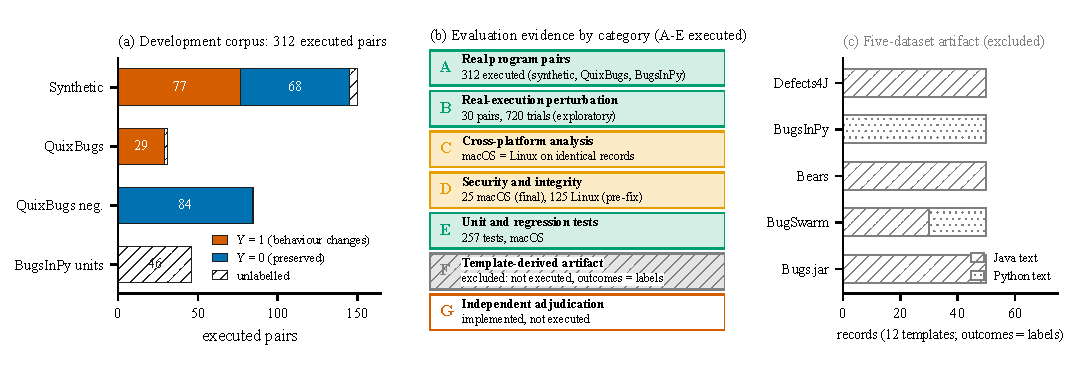
\includegraphics[width=\textwidth]{figures/fig_evidence_landscape.pdf}
\caption{Evidence landscape. (a) The executed development corpus by arm and construction label (data: \code{dev\_records.jsonl}). (b) Status of the seven evidence categories A--G. (c) The five-dataset artifact, shown hatched and grey because its records are template-generated with outcomes set from labels; it is invalid as external-validation evidence (outcomes set from labels, stub predictor, no benchmark executed, zero human verdicts), and no metric is derived from it.}
\label{fig:landscape}
\end{figure*}

\paragraph*{Consequences for interpretation} Three properties of the corpus limit what it can show.
\begin{enumerate}
\item All 13 false assurances under the V7-B gate are synthetic pairs.
\item In the QuixBugs arm, the same declared inputs produce both the label and the evidence, so a behaviour-changing pair almost always yields a witness. This understates risk there.
\item The corpus was examined repeatedly during design.
\end{enumerate}
The study is therefore a pilot on design-exposed data, not a validation.

\paragraph*{Study type and design controls} The paper combines a methodology contribution (Sections~\ref{sec:problem}--\ref{sec:trust}) with a pilot empirical study whose central predictive hypothesis was not supported. We frame it as a methodology and negative-results paper. Table~\ref{tab:controls} lists the confounders a reviewer should check, how the design handles each, and what remains. Three of them, development exposure, label provenance and the absence of a held-out benchmark, cannot be repaired with the existing data.

\begin{table*}[!t]
\caption{Design controls: how each threat to the empirical questions is handled and what remains uncontrolled.}
\label{tab:controls}
\centering
\scriptsize
\setlength{\tabcolsep}{3pt}
\renewcommand{\arraystretch}{1.08}
\begin{tabular}{|L{2.6cm}|L{6.4cm}|L{1.7cm}|L{4.9cm}|}
\hline
Threat & Control in the design & Status & Residual \\
\hline
Project dependence & Project-grouped CV folds; project-cluster bootstrap; ICC and design effect in the power analysis & Controlled & All QuixBugs pairs form one cluster (43.8\% of labels) \\
Development exposure & None possible on this corpus; stated as pilot; prediction lock prepared for a confirmatory study & Not controlled & Every result may be optimistic \\
Train--test leakage & Hyperparameters and thresholds chosen on inner folds; no project in both fitting and evaluation of a prediction & Controlled & Feature set designed on the whole corpus \\
Label provenance & Construction labels declared; worst-case risk reported; adjudication implemented & Not controlled & Labels are not adjudications under $(\obs,\budget)$ \\
Coverage differences & All comparisons at matched coverage $c^\ast$; random abstention B6 as reference (Prop.~\ref{prop:random}) & Controlled & $c^\ast$ fixed by the predecessor; matched point is transductive \\
Threshold selection & Inner-fold cluster-bootstrap thresholds; frozen-threshold study on held-out projects & Controlled & Deployable thresholds issued nothing or missed targets \\
Multiple comparisons & Holm within the pre-registered three-test family and within an eight-contrast family & Controlled & -- \\
Repeated perturbation trials & Trials reported as counts per property; no test pools trials across records & Controlled & Counts are descriptive only \\
Seeds & Five fold assignments reported separately, not pooled & Controlled & Sign of the primary contrast varies \\
Platform & Analysis repeated on macOS and Linux & Partly & Collection platform unrecorded; one environment id \\
Observation boundary & Four channels declared; risk is boundary-relative (Prop.~\ref{prop:mono}) & Declared & Not varied \\
Execution budget & Fixed collector configuration; P5 varies repeat counts & Partly & Adjudication budget undefined for construction labels \\
Single language & -- & Not controlled & Python only \\
\hline
\end{tabular}
\end{table*}

\subsection{Baselines and Ablations}
Table~\ref{tab:baselines} defines the comparators. All of them are evaluated on the same 258 labelled pairs with the same denominators.

\begin{table}[!t]
\caption{Baselines and ablations. ``Labels'' marks comparators fitted on labels (within training folds only).}
\label{tab:baselines}
\centering
\scriptsize
\setlength{\tabcolsep}{2.5pt}
\begin{tabular}{|c|L{4.4cm}|c|L{1.6cm}|}
\hline
Id & Definition & Labels & Role \\
\hline
B1 & Plain differential testing: \NDO{} unless a witness exists (``all inputs agree'') & No & Practice baseline \\
B2 & B1; a witness must be deterministic, a quarantined input yields \INS{} & No & Repetition \\
B3 & V7-B sufficiency gate (predecessor's fixed verdict) & No & Predecessor; sets $c^\ast$ \\
B4 & \NDO{} iff full activation and the branch-coverage floor hold & No & Coverage rule \\
B5 & B1, but \NDO{} only under full activation & No & Coverage rule \\
B6 & B1-issuable pairs abstained at random to $c^\ast$ (1{,}000 draws) & No & Chance reference (Prop.~\ref{prop:random}) \\
B7 & Logistic model on activation and branch coverage & Yes & Primary comparator \\
B8 & Full \cec{}: 15 profile features plus \ers{} responses & Yes & Proposed \\
B9 & \cec{} without \ers{}: 15 profile features & Yes & \ers{} ablation \\
-- & Coverage + multiplicity; multiplicity only & Yes & Multiplicity ablations \\
\hline
\end{tabular}
\end{table}

\subsection{Metrics and Matched Coverage}
For rule baselines we report coverage $\hat\cov$ (the share of the 258 labelled pairs issued \NDO{}) and observed risk $\hat\R$ (the share of issued \NDO{} verdicts with $Y{=}1$), together with worst-case risk that counts unlabelled \NDO{} pairs as false assurances. For calibrated models we report out-of-fold Brier score, log loss, logistic calibration slope, reliability diagrams and risk--coverage curves.

The primary comparison fixes coverage at $c^\ast=61/258=0.236$, the coverage of the V7-B gate (Algorithm~\ref{alg:matched}). Ranking happens within each outer fold, because risks from different fold models are not comparable, and ties are issued fractionally so that the operating point is exact. This is a transductive diagnostic of ranking quality, not a deployable threshold. Deployable thresholds are evaluated separately with Algorithm~\ref{alg:cec} at $\alpha\in\{0.10,0.15\}$.

\begin{algorithm}[!t]
\caption{Matched-coverage risk}
\label{alg:matched}
\small
\begin{algorithmic}[1]
\Statex \textit{Implements:} \bcode{stats.matched\_risk}
\Require out-of-fold scores $s$, eligibility, labels $Y$, target $c^\ast$, optional bootstrap weights $w$ (default 1)
\State $k\gets c^\ast\cdot\sum_k w_k$ \Comment{weighted number of verdicts to issue}
\State order eligible pairs by $s$ ascending; group equal scores
\State issue whole groups while the issued weight is below $k$; issue the boundary group fractionally
\If{eligible weight $<k$} \Return undefined \Comment{dropped resample; share reported as ``valid''}
\EndIf
\State \Return $\sum(\text{issued fraction}\times w\times Y)\,/\,k$
\end{algorithmic}
\end{algorithm}

\subsection{Statistical Methodology}
\begin{itemize}
\item \emph{Cross-validation.} Calibrated models are evaluated by project-grouped five-fold cross-validation, so no project contributes to both fitting and evaluating the same prediction. Hyperparameters and thresholds are selected on inner folds only.
\item \emph{Uncertainty.} We use a percentile project-cluster bootstrap with 10{,}000 resamples. Paired contrasts are bootstrapped jointly, and we report the share of resamples in which a matched-coverage contrast is defined.
\item \emph{Tests and multiplicity.} Bootstrap $p$-values are one-sided, with the alternative that B8 has lower risk or log loss. The pre-registered primary family (B8 vs.\ B7, B3, B6) is Holm-adjusted. We also report a wider family of eight contrasts per policy with Holm adjustment.
\item \emph{Seeds.} Five fold assignments are replicates over the same pairs; they are not pooled for inference.
\item \emph{Power.} We report the minimum detectable paired difference at 80\% power and two-sided $\alpha=0.05$, using the intra-cluster correlation of the V7-B \NDO{} set.
\item \emph{Interpretation.} Non-significance is never read as equivalence. No equivalence margin was pre-registered, so no equivalence test is reported.
\end{itemize}

\paragraph*{Pre-registered hypotheses} The analysis plan, fixed before evaluation, specified four hypotheses.
\begin{itemize}
\item \emph{H2 (primary).} At matched coverage, B8 reduces risk relative to B7 by at least 5 points, with a one-sided 97.5\% lower bound above zero.
\item \emph{H1a.} The full profile improves out-of-fold log loss over coverage-only calibration (B9 vs.\ B7).
\item \emph{H3.} \ers{} features improve log loss and matched risk over the profile alone (B8 vs.\ B9).
\item \emph{H4.} Calibration slope and intercept; declared not assessable without an independent holdout.
\end{itemize}
